\chapter{Lógicas de Descrição}
\label{chap:logicas}

\lettrine{A}{} área de Inteligência Artificial é composta por diversas subáreas. Uma delas é a de Representação de Conhecimento, que cuida de construir formalismos adequados para expressar conhecimento sobre um domínio. Tal área estuda entidades inteligentes, que possuem algum tipo de conhecimento e precisam fazer inferências a partir dele.

Existe um consenso, já mencionado no \autoref{chap:ontologias}, de que linguagens formais são uma maneira boa de caracterizar axiomas lógicos para a modelagem de uma ontologia. O principal formalismo utilizado para representar conhecimento, com um cuidado especial para as terminologias, são as Lógicas de Descrição (doravante, LD).

Essas lógicas são um subconjunto da Lógica de Primeira Ordem (a partir de agora, LPO), que por sua vez, estende a Lógica Proposicional. As LD são utilizadas por sua expressividade. Para anotar que uma \texttt{Cancao} ou um \texttt{HinoNacional} são uma \texttt{Musica}, usando a ontologia que está sendo desenvolvida neste trabalho, podem ser utilizadas as seguintes sentenças, usando as lógicas até agora citadas:

\begin{table}[H]
	\centering
	\begin{tabular}{|l|l|l}
		\cline{1-2}
		Lógica                           & Sentença                                                                             & \\ \cline{1-2}
		Proposicional                    & $c \lor h \to m$                                                                     & \\ \cline{1-2}
		de Primeira Ordem                & $\forall x(\texttt{Cancao}(x) \lor \texttt{HinoNacional}(x) \to \texttt{Musica}(x))$ & \\ \cline{1-2}
		de Descrição ($ \mathcal{ALC} $) & \texttt{Cancao} $\sqcup$ \texttt{HinoNacional} $\sqsubseteq$ \texttt{Musica}         & \\ \cline{1-2}
	\end{tabular}
\caption{A mesma sentença expressa em diferentes lógicas}
\end{table}

Pode-se observar que a notação da LD permite que o entendimento de suas sentenças seja feito usando a Teoria dos Conjuntos. A última sentença da tabela leva a entender que a ''união'' dos ''conjuntos'' \texttt{Cancao} e \texttt{HinoNacional} está contida no ''conjunto'' \texttt{Musica}.

No entanto, é necessário certo cuidado com essa compreensão. Os conceitos, na verdade, são mapeados a conjuntos. Esses, por sua vez, são subconjuntos de um domínio. Quem faz o mapeamento é uma função de interpretação. As definições necessárias para o entendimento desse parágrafo estão diluídas pelo capítulo.

\section{Conceitos, papéis e indivíduos}

As LD possuem um jeito próprio de organizar o conhecimento. Elas usam três definições para retratar o que é desejado \cite{logicaMatos}. Cada uma delas é utilizada na construção de uma ontologia. São, a seguir:

\begin{description}
	\item[Conceitos] Também chamados de classes, representam um conjunto de indivíduos. Nas ontologias, são equivalentes às Classes.
	\item[Papéis] Podem ser denotados como propriedades. Retratam as relações binárias que existem entre os indivíduos. Basicamente, são as Relações de uma ontologia. Alguns papéis podem ter uma função de caracterização, ou seja, definindo alguns atributos para o conceito. Tal função corresponde a uma Propriedade de uma Classe, em uma ontologia.
	\item[Indivíduos] Representam os particulares que existem dentro de um Conceito. Para as ontologias, são as Instâncias.
\end{description}

Logo, uma LD é definida por uma tripla $ (N_C, N_R, N_I) $, onde $ N_C $ é um conjunto de Conceitos atômicos, $ N_R $ é um conjunto de Papéis atômicos e $ N_I $ é um conjunto de nomes de indivíduos.

Feita essa distinção, o conhecimento em uma ontologia é dividido em duas partes, com as LD. A primeira delas é a \textit{TBox}. Ela se refere ao conhecimento terminológico, ou seja, o conhecimento intensional do domínio. Nela ficam os conceitos, as propriedades e as restrições.

A outra parte é a \textit{ABox}, e nela fica o conhecimento assertivo, ou seja, o conhecimento extensional. Ela contém as asserções sobre as instâncias, ou seja, como eles se encaixam nas definições explícitas na \textit{TBox}.

\section{$\mathcal{ALC}$ e outras linguagens}

As pesquisas na área de Representação de Conhecimento levaram à confecção das chamadas Linguagens Terminológicas de Representação. Uma delas é a KL-ONE de Brachman, que possui uma semântica clara, além de separar o conhecimento assertivo e terminológico. %Citar o home

Tais estudos levaram ao desenvolvimento da $\mathcal{ALC}$. Essa linguagem, cuja sigla significa \textit{Attributive Concept Language with Complements}, é uma das Lógicas de Descrição mais básicas que existem, embora seja uma das mais utilizadas para as atividades que envolvem raciocínio lógico. 

Ela contempla os seguintes construtores, para quaisquer conceitos \texttt{A} e \texttt{B} e qualquer papel \texttt{r}:

\begin{table}[H]
	\centering
	\begin{tabular}{|c|c|l}
		\cline{1-2}
		Nome               & Notação                          &  \\ \cline{1-2}
		Conceito Universal & $ \top $                         &  \\ \cline{1-2}
		Conceito Vazio     & $ \bot $                         &  \\ \cline{1-2}
		Conceito Atômico   & \texttt{A}                       &  \\ \cline{1-2}
		Negação            & $ \neg $\texttt{A}               &  \\ \cline{1-2}
		União              & \texttt{A} $ \sqcup $ \texttt{B} &  \\ \cline{1-2}
		Intersecção        & \texttt{A} $ \sqcap $ \texttt{B} &  \\ \cline{1-2}
		Universal          & $\forall$ \texttt{r.A}           &  \\ \cline{1-2}
		Existencial        & $\exists$ \texttt{r.A}           &  \\ \cline{1-2}
	\end{tabular}
	\caption{Construtores da Lógica $ \mathcal{ALC} $}
\end{table}

Essa representação também permite que sejam escritos axiomas terminológicos, tais como a subsunção, denotada por $ \texttt{A} \sqsubseteq \texttt{B} $, e a equivalência, caracterizada como $ \texttt{A} \equiv \texttt{B} $ e que significa $ \texttt{A} \sqsubseteq \texttt{B} $ e $ \texttt{B} \sqsubseteq \texttt{A} $. Para o conhecimento assertivo também existem axiomas, tanto para conceitos ($\texttt{A}(x)$), quanto para papéis ($\texttt{r}(x,y)$).

A linguagem $\mathcal{ALC}$ permite que seja feita a negação de conceitos complexos (não-atômicos). Tal propriedade permite descobrir, por exemplo, se algum conceito é satisfatível. Usando o símbolo $ \sim $ para demonstrar equivalência, teremos que:

\begin{itemize}
	\item $ \neg(\forall r.\texttt{A}) \sim \exists r.\neg \texttt{A}$ 
	\item $ \neg(\exists r.\texttt{A}) \sim \forall r.\neg \texttt{A}$ 
	\item $ \neg(\texttt{A} \sqcup \texttt{B}) \sim \neg \texttt{A} \sqcap \neg \texttt{B}$ 
	\item $ \neg(\texttt{A} \sqcap \texttt{B}) \sim \neg \texttt{A} \sqcup \neg \texttt{B}$ 
	\item $ \neg \neg \texttt{A} \sim \texttt{A} $
\end{itemize}

A partir de sua constituição, é possível definir três sublinguagens da $\mathcal{ALC}$ \cite{logicaSchmidt}, que são descritas a seguir.

\begin{itemize}
	\item $\mathcal{ALE}$: permite a descrição de conceitos simples sem a utilização de uniões; 
	\item $\mathcal{ALU}$: deixa apenas conceitos simples serem descritos e restringe as quantificações de papéis existenciais à forma $ \exists\texttt{r}.\top $;
	\item $\mathcal{AL}$: é a intersecção das sublinguagens acima.
\end{itemize}

Os nomes das sublinguagens acima são derivados da seguinte maneira: $ \mathcal{ALU} $ vem da junção de $ \mathcal{AL} $ com uniões, $ \mathcal{ALE} $ é a $ \mathcal{AL} $ acrescida de quantificadores existenciais. A própria $ \mathcal{ALC} $ é uma extensão da $ \mathcal{AL} $ com adição de complementos (negações) para qualquer conceito, seja ele atômico ou complexo. 

Nota-se que a sigla que representa o nome de uma linguagem expressa as características que ela possui.
A $ \mathcal{ALC} $ é base para outras linguagens mais expressivas, que são construídas a partir de sua extensão. Algumas delas são:

\begin{itemize}
	\item $ \mathcal{S} $: linguagem $ \mathcal{ALC} $ com papéis transitivos;
	\item $ \mathcal{F} $: propriedades funcionais;
	\item $ \mathcal{N} $: restrição numérica;
	\item $ \mathcal{C} $: negação de conceitos complexos;
	\item $ \mathcal{U} $: união de conceitos;
	\item $ \mathcal{E} $: quantificação existencial completa;
	\item $ \mathcal{Q} $: restrição numérica qualificada;
	\item $ \mathcal{O} $: nominal;
	\item $ \mathcal{H} $: hierarquia de papéis;
	\item $ \mathcal{I} $: propriedades inversas;
	\item $ \mathcal{N} $: restrições de cardinalidade;
	\item $ ^\mathcal{(D)} $: usa propriedades de tipo de dados.
\end{itemize}

Com essa nomenclatura, pode-se dar duas linguagens como exemplo\cite{logicaResina}. Uma delas é a $ \mathcal{SHIF}^\mathcal{(D)} $, que engloba a $ \mathcal{ALC} $ e, ainda, hierarquia de papéis, propriedades inversas, transitivas e funcionais e tipos de dados.

Uma outra é a lógica $ \mathcal{SHOIN}^\mathcal{(D)}$, que envolve a  $ \mathcal{SHIF}^\mathcal{(D)} $ e restrições de cardinalidade em papéis.

\section{Interpretação e Consequência Lógica}

Uma interpretação $ \mathcal{I} = (\Delta^{\mathcal{I}}, \cdot^{\mathcal{I}})$ consiste em um conjunto domínio ($ \Delta^{\mathcal{I}} $) e uma função de interpretação $ \cdot^{\mathcal{I}} $ que atribui a toda descrição de conceito um subconjunto de $ \Delta^{\mathcal{I}} $, seguindo as seguintes equações\cite{logicaHorrocks}:

\begin{itemize}
	\item $ \top^\mathcal{I} = \Delta^\mathcal{I} $
	\item $ \bot^\mathcal{I} = \emptyset $
	\item $ (\neg \texttt{A})^\mathcal{I} = \Delta^\mathcal{I} \setminus \texttt{A}^\mathcal{I}  $
	\item $(\texttt{A} \sqcup \texttt{B})^\mathcal{I} = \texttt{A}^\mathcal{I} \cup \texttt{B}^\mathcal{I}$  
	\item $(\texttt{A} \sqcap \texttt{B})^\mathcal{I} = \texttt{A}^\mathcal{I} \cap \texttt{B}^\mathcal{I}$
	\item $(\exists \texttt{r.A})^\mathcal{I} = \{a \in \Delta^\mathcal{I}\text{ }|\text{ existe } b \in \Delta^\mathcal{I} \text{ tal que } (a, b) \in \texttt{r}^\mathcal{I}\}$  
	\item $(\forall \texttt{r.A})^\mathcal{I} = \{a \in \Delta^\mathcal{I}\text{ }| \text{ para todo } b \in \Delta^\mathcal{I}\text{, se } (a, b) \in \texttt{r}^\mathcal{I}\text{, então } b \in \texttt{A}^\mathcal{I}\}$
\end{itemize}

Com isso, podemos ver que uma interpretação $ \mathcal{I} $ satisfaz:

\begin{multicols}{2}
	\begin{itemize}
		\item \texttt{A} $ \equiv $ \texttt{B} se e somente se $ \texttt{A}^\mathcal{I} $ = $ \texttt{B}^\mathcal{I} $ 
		\item \texttt{A} $ \sqsubseteq $ \texttt{B} se e somente se $ \texttt{A}^\mathcal{I} \subseteq \texttt{B}^\mathcal{I} $
		\item a \textit{TBox} $ \mathcal{T} $ se e somente se satisfaz todos os elementos de $ \mathcal{T} $
		\item $ \texttt{A}(a) $ se e somente se $ a^\mathcal{I} \in A^\mathcal{I} $
		\item $ \texttt{r}(a, b) $ se e somente se $ (a^\mathcal{I}, b^\mathcal{I}) \in \texttt{r}^\mathcal{I} $
		\item a \textit{ABox} $ \mathcal{A} $ se e somente se satisfaz todos os elementos de $ \mathcal{A} $
	\end{itemize}
\end{multicols}

Uma Base de Conhecimento $ \mathcal{ALC} $ é um par $ \Sigma = (\mathcal{T}, \mathcal{A}) $ onde $ \mathcal{T} $ é uma \textit{TBox} e $ \mathcal{A} $, uma \textit{TBox}. Logo, pode ser dito que uma interpretação $ \mathcal{I} $ é um modelo de $ \Sigma $ se satisfaz $ \mathcal{T} $ e $ \mathcal{A} $. Uma base de conhecimento $ \Sigma $ é satisfatível se admite um modelo.

Com isso, podemos definir Consequência Lógica como $ \Sigma \models \phi $ se todo modelo de $ \Sigma $ é um modelo de $ \phi $. Na ontologia deste texto, isso pode ser aplicado da seguinte maneira, sendo:

\begin{itemize}
	\item $ \Sigma = (\mathcal{T}, \mathcal{A}) $, onde:
	\begin{itemize}
		\item $ \mathcal{T} $ é a \textit{TBox}: $ \texttt{HinoNacional} \sqsubseteq \texttt{Musica} $
		\item $ \mathcal{A} $ é a \textit{ABox}: \texttt{HinoNacional(hinoNacionalBrasileiro)}
	\end{itemize}
\end{itemize}

É possível observar que $ \Sigma \models \texttt{Musica(hinoNacionalBrasileiro)} $ será uma consequência lógica.

\section{Equivalências com a Lógica de Primeira Ordem}

As LD, como definido anteriormente, são um subconjunto das LPO. Portanto, toda e qualquer expressão expressa nessa linguagem terá um equivalente em LPO. 

Tal relação se estende até às definições que ela utiliza em sua constituição. Os conceitos, papéis e indivíduos acima citados, correspondem, respectivamente, a predicados unários, predicados binários e constantes em Lógica de Primeira Ordem.

Com essa elucidação, é possível elaborar uma tabela que mostra as principais equivalências entre LD e LPO, com intenção de usá-la para uma eventual tradução entre as lógicas. Definindo $t_x$ como a interpretação em $x$ de uma sentença, já que é necessária uma variável livre para a tradução, teremos:

\begin{table}[H]
	\centering
	\begin{tabular}{|c|c|c|c|l}
		\cline{1-4}
		Conceito     & LD                                    & Tradução                                 & LPO                                              &  \\ \cline{1-4}
		Classe       & \texttt{A}                            & $t_x(\texttt{A})$                        & $A(x)$                                           &  \\ \cline{1-4}
		União        & \texttt{A} $ \sqcup $ \texttt{B}      & $t_x(\texttt{A} \sqcup \texttt{B})$      & $A(x) \lor B(x)$                                 &  \\ \cline{1-4}
		Intersecção  & \texttt{A} $ \sqcap $ \texttt{B}      & $t_x(\texttt{A} \sqcap \texttt{B})$      & $A(x) \land B(x)$                                &  \\ \cline{1-4}
		Universal    & $\forall$ \texttt{r.A}                & $t_x(\forall \texttt{r.A})$              & $\forall y(r(x,y) \to t_y(A))$                   &  \\ \cline{1-4}
		Existencial  & $\exists$ \texttt{r.A}                & $t_x(\exists \texttt{r.A})$              & $\exists y(r(x,y) \land t_y(A))$                 &  \\ \cline{1-4}
		Subsunção    & \texttt{A} $ \sqsubseteq $ \texttt{B} & $t_x(\texttt{A} \sqsubseteq \texttt{B})$ & $\forall x(t_x(A) \to t_x(B))$                   &  \\ \cline{1-4}
		Equivalência & \texttt{A} $ \equiv $ \texttt{B}      & $t_x(\texttt{A} \equiv \texttt{B})$      & $\forall x(t_x(A) \longleftrightarrow t_x(B))$   &  \\ \cline{1-4}
	\end{tabular}
	\caption{Tabela para tradução entre LD e LPO}
\end{table}

Usando a ontologia de música como exemplo, pode-se ver como essa tradução é aplicada:

\begin{enumerate}
	\item \texttt{Pop} $ \sqsubseteq $ \texttt{Cancao} vira $\forall x(\texttt{Pop}(x) \to \texttt{Cancao}(x))$.
	\item \texttt{Cancao} $ \sqcup $ \texttt{HinoNacional} $ \sqsubseteq $ \texttt{Musica} é traduzida como $\forall x(\texttt{Cancao}(x) \lor \texttt{HinoNacional}(x) \\ \to \texttt{Musica}(x))$.
	\item $ \forall $ \texttt{canta.Musica} $ \sqsubseteq $ \texttt{Cantor} corresponde a $ \forall x(\forall y(\texttt{canta}(x,y) \to \texttt{Musica}(y)) \to \\ \texttt{Cantor}(x)) $.
	\item $ \exists $ \texttt{canta.Pop} $ \sqsubseteq $ \texttt{Cantor} $ \sqcap $ \texttt{Compositor} equivale a $ \forall x (\exists y(\texttt{canta}(x,y) \land \texttt{Pop}(y)) \to \\ \texttt{Cantor}(x) \land \texttt{Compositor}(x))$.
\end{enumerate}


\section{Consistência}

Após uma Base de Conhecimento ser feita, é necessário que ela seja consistente, ou seja, ela não pode se contradizer. A inconsistência acontece quando a inferência de um conceito e sua negação, ao mesmo tempo, é possível. 

Para verificar tal propriedade, podem ser aplicadas as regras de \textit{tableau} para Lógicas de Descrição. Com elas, é possível determinar de maneira algorítmica a consistência de uma Base de Conhecimento. São elas:

\begin{description}
	\item[Regra \texttt{E} (ou \textit{$ \sqcap $-rule})] Se $(\texttt{A} \sqcap \texttt{B})(a)$ está em $ \mathcal{A} $, mas \texttt{A}$ (a) $ e \texttt{B}$ (a) $ não estão os dois em $ \mathcal{A} $, então a \textit{ABox} $ \mathcal{A} $ será acrescida de \texttt{A}$ (a) $ e \texttt{B}$ (a) $.
	\item[Regra \texttt{OU} (ou \textit{$ \sqcup $-rule})] Quando $(\texttt{A} \sqcup \texttt{B})(a)$ está em $ \mathcal{A} $, mas nem \texttt{A}$ (a) $ nem \texttt{B}$ (a) $ está em $ \mathcal{A} $, então à \textit{ABox} $ \mathcal{A} $ será incluído \texttt{A}$ (a) $ ou \texttt{B}$ (a) $.
	\item[Regra \texttt{EXISTE} (ou \textit{$ \exists $-rule})] Se $(\exists \texttt{r.A})(a)$ está em $ \mathcal{A} $, e não há nenhum indivíduo $ c $ tal que \texttt{r}$ (a,c) $ e \texttt{A}$ (c) $ estejam em $ \mathcal{A} $, então tanto \texttt{r}$ (a,b) $ quanto \texttt{A}$ (b) $ serão adicionados a $ \mathcal{A} $, onde $ b $ é um novo indivíduo.
	\item[Regra \texttt{PARA TODO} (ou \textit{$ \forall $-rule})] Quando se $(\forall \texttt{r.A})(a)$ e \texttt{r}$ (a,b) $ estão em $ \mathcal{A} $, mas \texttt{A}$ (b) $ não está, esse último será colocado em $ \mathcal{A} $.  
\end{description}

Para descobrir se uma fórmula é insatisfatível, basta aplicar essas regras na sentença lógica. Se, no final, um \textit{Clash} (choque) for alcançado, isto é, quando temos um conceito e sua negação na \textit{ABox}, a sentença é insatisfatível.

Koubarakis \cite{logicaKoubarakis} deu um exemplo para aplicar essas regras:

	\begin{figure}[H]
		\centering
		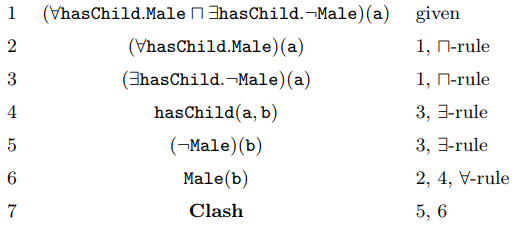
\includegraphics[width=0.6\textwidth]{Capitulos/Logicas/tableau}
		\caption{Exemplo de aplicação das regras de \textit{Tableau}}
	\end{figure}

Note que nesse exemplo não há uso da \textit{$ \sqcup $-rule}. Quando ela é usada, são criados dois ramos. Para que a fórmula seja insatisfazível, os dois devem resultar em choque (\textit{Clash}).

Para verificar que sentenças no estilo $ \texttt{C} \sqsubseteq \texttt{D} $ são válidas, deve ser verificada a satisfazibilidade de $ \texttt{C} \sqcap \neg \texttt{D} $. Se essa última for insatisfatível, a primeira é consequência lógica da base de conhecimento.